\documentclass[12pt, twoside]{article}
\usepackage[letterpaper, margin=1in, headsep=0.5in]{geometry}
\usepackage[english]{babel}
\usepackage[utf8]{inputenc}
\usepackage{amsmath}
\usepackage{amsfonts}
\usepackage{amssymb}
\usepackage{tikz}
\usetikzlibrary{quotes, angles}
\usepackage{graphicx}
\usepackage{enumitem}
\usepackage{multicol}

\newif\ifmeta
\metatrue %print standards and topics tags

\title{Regents Geometry}
\author{Chris Huson}
\date{October 2021}

\usepackage{fancyhdr}
\pagestyle{fancy}
\fancyhf{}
\renewcommand{\headrulewidth}{0pt} % disable the underline of the header
\raggedbottom


\fancyhead[LE]{\thepage}
\fancyhead[RO]{\thepage \\ Name: \hspace{4cm} \,\\}
\fancyhead[LO]{BECA / Dr. Huson / Geometry 04 Analytic Geometry}

\begin{document}

\subsubsection*{4.9 Review: Transversals and angles}
\begin{enumerate}
\item Do Now: Given two parallel lines and a transversal, as shown, with $m\angle 8 = 117^\circ$.
  \begin{multicols}{2}
    \begin{enumerate}[itemsep=0.5cm]
      \item What angle is corresponding to $\angle 8$?
      \item What angle is alternate exterior to $\angle 8$?
      \item Find $m\angle 2$ \vspace{1cm}
    \end{enumerate}
    \begin{flushright}
      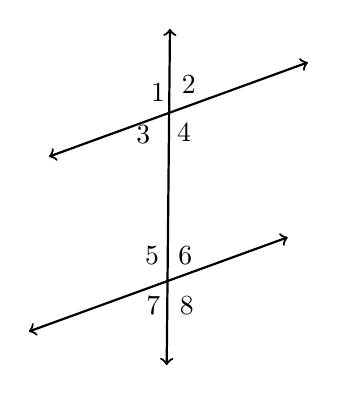
\begin{tikzpicture}[scale=1,rotate=20]
      \draw [<->, thick] (3.5,2)--(7,2);
      \draw [<->, thick] (2.5,0)--(6,0);
      \draw [<->, thick] (4,-1)--(5.5,3);
      \node at (4.5,0.3) [left]{$5$};
      \node at (4.5,0.3) [right]{$6$};
      \node at (4.3,-0.3) [left]{$7$};
      \node at (4.3,-0.3) [right]{$8$};
      \node at (5.2,2) [above left]{$1$};
      \node at (5.2,2.1) [above right]{$2$};
      \node at (5,2) [below left]{$3$};
      \node at (5.1,2) [below right]{$4$};
    \end{tikzpicture}
  \end{flushright}
  \end{multicols}

\item Find $m\angle 1$ given two parallel lines and a transversal, with
  \begin{multicols}{2}
  $\displaystyle m\angle 2 = 2x+41$ \hspace{0.75cm}$\displaystyle m\angle 7 = \frac{1}{2}(5x+5)$
\begin{flushright}
  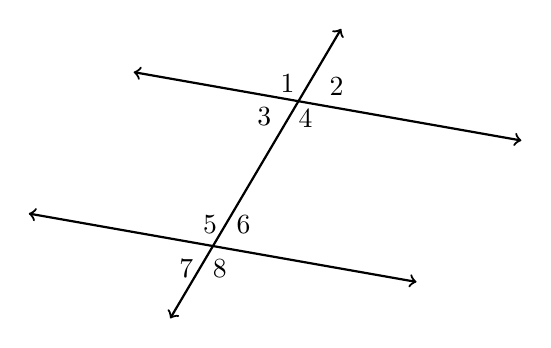
\begin{tikzpicture}[scale=1,rotate=-10]
    \draw [<->, thick] (3,2)--(8,2);
    \draw [<->, thick] (2,0)--(7,0);
    \draw [<->, thick] (4,-1)--(5.5,3);
    \node at (4.5,0.3) [left]{$5$};
    \node at (4.5,0.3) [right]{$6$};
    \node at (4.3,-0.3) [left]{$7$};
    \node at (4.3,-0.3) [right]{$8$};
    \node at (5.2,2) [above left]{$1$};
    \node at (5.4,2) [above right]{$2$};
    \node at (4.9,2) [below left]{$3$};
    \node at (5,2) [below right]{$4$};
  \end{tikzpicture}
\end{flushright} 
\end{multicols} \vspace{2cm}

\item As shown below, two lines intersect making four angles: $\angle 1$, $\angle 2$, $\angle 3$, and $\angle 4$. Given that $m\angle 1= x+32$ and $m\angle 3=2x-8$, find $m\angle 1$.
  \begin{flushright}
    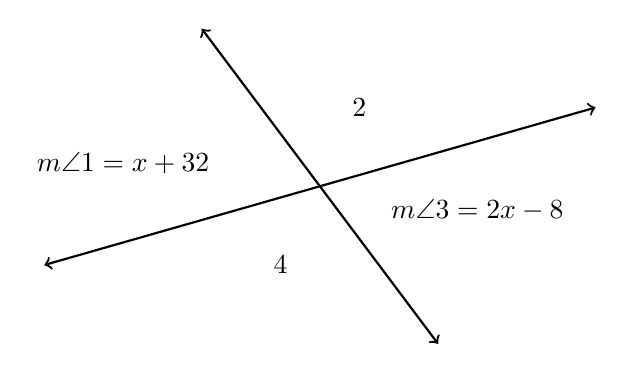
\begin{tikzpicture}[scale=1, rotate=0]
      \draw [<->, thick] (1,-1)--(8,1);
      \draw [<->, thick] (3,2)--(6,-2);
      \node at (2,.3){$m\angle 1= x+32$};
      \node at (6.5,-.3){$m\angle 3=2x-8$};
      \node at (5,1){2};
      \node at (4,-1){4};
    \end{tikzpicture}
    \end{flushright}

\newpage
\item An angle bisector is shown below, with $\overrightarrow{PR}$ bisecting $\angle QPS$. Given $m\angle QPR = 6x-12$ and $m\angle QPS = 10x+4$, find $m\angle QPS$.
    \begin{flushright}
    \begin{tikzpicture}[scale=0.6, rotate=30]
      \draw [<->, thick] (230:5)node[left]{$Q$} 
      --(0,0)node[above right]{$P$}
      --(110:6)node[above right]{$S$}--(110:7);
      \draw [->, thick] (0,0)--(170:7)node[below right]{$R$};
      %\draw [fill] (0,0) circle [radius=0.05] node[below]{$A$};
      %\draw [fill] (5,0) circle [radius=0.05] node[below]{$B$};
    \end{tikzpicture}
    \end{flushright}

    \item Graph and label $\triangle CAT$. Calculate the lengths of its sides. $C(1,2)$, $A(10,8)$, $T(10,2)$.
    \begin{flushleft}
      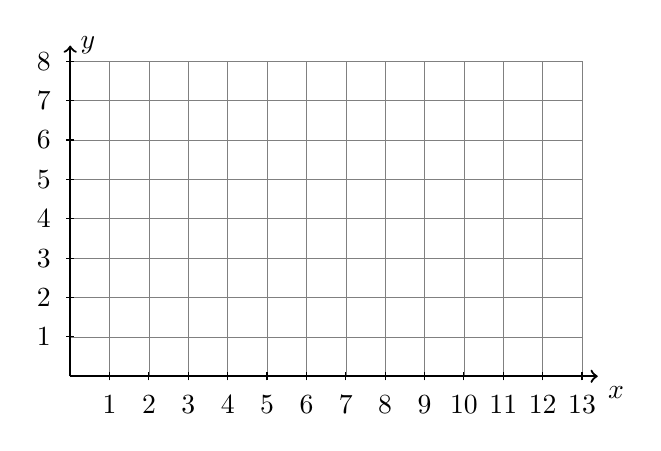
\begin{tikzpicture}[scale=.5]
        \draw [help lines] (0,0) grid (13,8);
        \draw [thick, ->] (0,0) -- (13.4,0) node [below right] {$x$};
        \draw [thick, ->] (0,0)--(0,8.4) node [right] {$y$};
        \foreach \x in {1,...,13}
        \draw[shift={(\x,0)}] (0pt,-3pt)--(0pt,3pt) node[below=5pt] {$\x$};
        \foreach \y in {1,...,8}
        \draw[shift={(0,\y)}] (-3pt,0pt)--(3pt,0pt) node[left=5pt] {$\y$};
      \end{tikzpicture}
    \end{flushleft}
    
    \item The base of a right triangle is 8 centimeters long and its hypotenuse is 10 cm. Find its height, $x$ cm.
    \begin{flushright}
      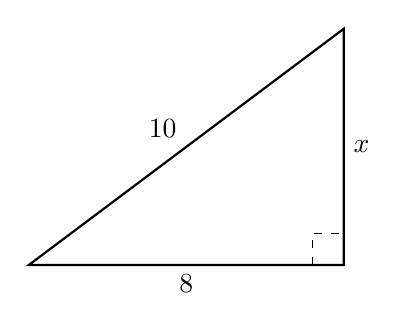
\begin{tikzpicture}[scale=1]
        \node at (2,1.5)[above left]{10};
        \node at (4,1.5)[right]{$x$};
        \node at (2,0)[below]{8};
        \draw [thick] (0, 0)--(4, 0)--(4, 3)--cycle;
        \draw [dashed] (4,0)++(-0.4,0)-- ++(0,0.4)-- +(0.4,0);
      \end{tikzpicture}
    \end{flushright}
 

\end{enumerate}
\end{document}